\section{Hardware}
Um eine volle Alternative zu jeglichen Taschenrechnern bieten zu können, musste eine entsprechende Hardware entwickelt werden, auf der man problemlos unsere Software bedienen kann. Dazu brauchten wir eine Recheneinheit, einen Display, eine für den Benutzer einfach zu bedienende Eingabemöglichkeit und ein passendes Gehäuse.\\

Von Anfang an war klar, dass die Hauptrecheneinheit unseres Prototypen fähig sein musste, den Rechenaufwand unserer Software problemlos zu bewältigen. Ein weiteres wichtiges Kriterium war, einen kleinen Formfarktor einhalten zu können, um zu garantieren, dass unsere Einheit in einem handlichen Gehäuse Platz findet. Beiden Punkten zugleich wird lediglich ein \textit{single-board-computer} gerecht, er vereint hohe Rechenleistung mit minimalem Platzaufkommen.\\

Das Display musste groß genug sein, um dem Benutzer genug Platz zu bieten, seine Berechnungen und Notizen durchzuführen. Allerdings war auch wichtig darauf zu achten, dass es nicht zu groß war um nicht die Portabilität unseres Gerätes einzuschränken.\\

Mittels dem \textit{Touchscreen} ist es möglich, Berechnungen einzugeben sowie Mitschriften zu tätigen. Er wird mithilfe eines Stiftes bedient.\\

Da der single-board-computer und Display einen relativ hohen Energiebedarf aufweisen, musste eine Hardware-Komponente her, welche beide je nach Bedarf aus-und-einschalten kann. Bei dieser Komponente war darauf zu achten, dass diese dem Gerät so wenig Energie wie möglich entzieht um eine lange \textit{Standby-Zeit} zu garantieren. Die Komponente kann auf Knopfdruck Display und Recheneinheit getrennt von einander stromlos machen.\\

\subsection{Recheneinheit}
Bei der großen Auswahl an single-board-computern entschieden wir und für den \textit{Raspberry Pi 3}, da dieser neben hervorragendem Treibersupport, den wir für unseren Touchscreen benötigen, durch eine für den Formfaktor sehr hohe Leistung überzeugt. Weiters ist bereits eine Wireless-LAN Schnittstelle verbaut, welche bei der Software-Installation sehr behilflich ist.\\
\\
Nach Installation der aktuellen Firmware auf dem Raspberry Pi war es nicht möglich den Touchscreen-Treiber zu kalibrieren, dieses Problem führte zu einigen Verzögerungen. Bis dieser Fehler auf Seiten der Raspberry Pi Software behoben ist, wird eine ältere Version, auf der der Touchscreen-Treiber noch problemlos kalibrierbar ist verwendet.\\
\\
Da das Betriebssystem der Recheneinheit auf einer SD-Karte installiert ist, und diese auch zum Booten verwendet wird, ist es wichtig diese SD-Karte in entsprechender Qualität auszuführen. Zu Beginn gab es einige Probleme hinsichtlich einer schlechten SD-Karte da diese andauernd Korruptions-Probleme hatte und aufgrund der geringen Lesegeschwindigkeit sehr lange brauchte um den Boot-Vorgang abzuschließen. Bei der jetzt verwendeten SD-Karte handelt es sich um ein Modell von SanDisk, welches mit einer nominalen Lesegeschwindigkeit von 95 Mbps überzeugt, nach der Umstellung auf die neue Karte gab es auch keine Korruptions-Probleme mehr.\\
\\
Für den Raspberry Pi wurde ein Python-Skript entwickelt welches auf ein Signal des \textit{Power-Button} auf GPIO Pin 23 wartet. Sobald ein Signal empfangen wird, fährt die Recheneinheit herunter und sendet nach dem Shutdown ein Signal auf GPIO Pin 24, welches dem Mikrocontroller der Power-Button Einheit mitteilt, dass die Recheneinheit erfolgreich heruntergefahren worden ist. Der Mikrocontroller macht darauf hin Display und Recheneinheit stromlos.\\
\\
Die GPIO-Pins des Raspberry Pi sind folgendermaßen aufgebaut:\\
\begin{center}
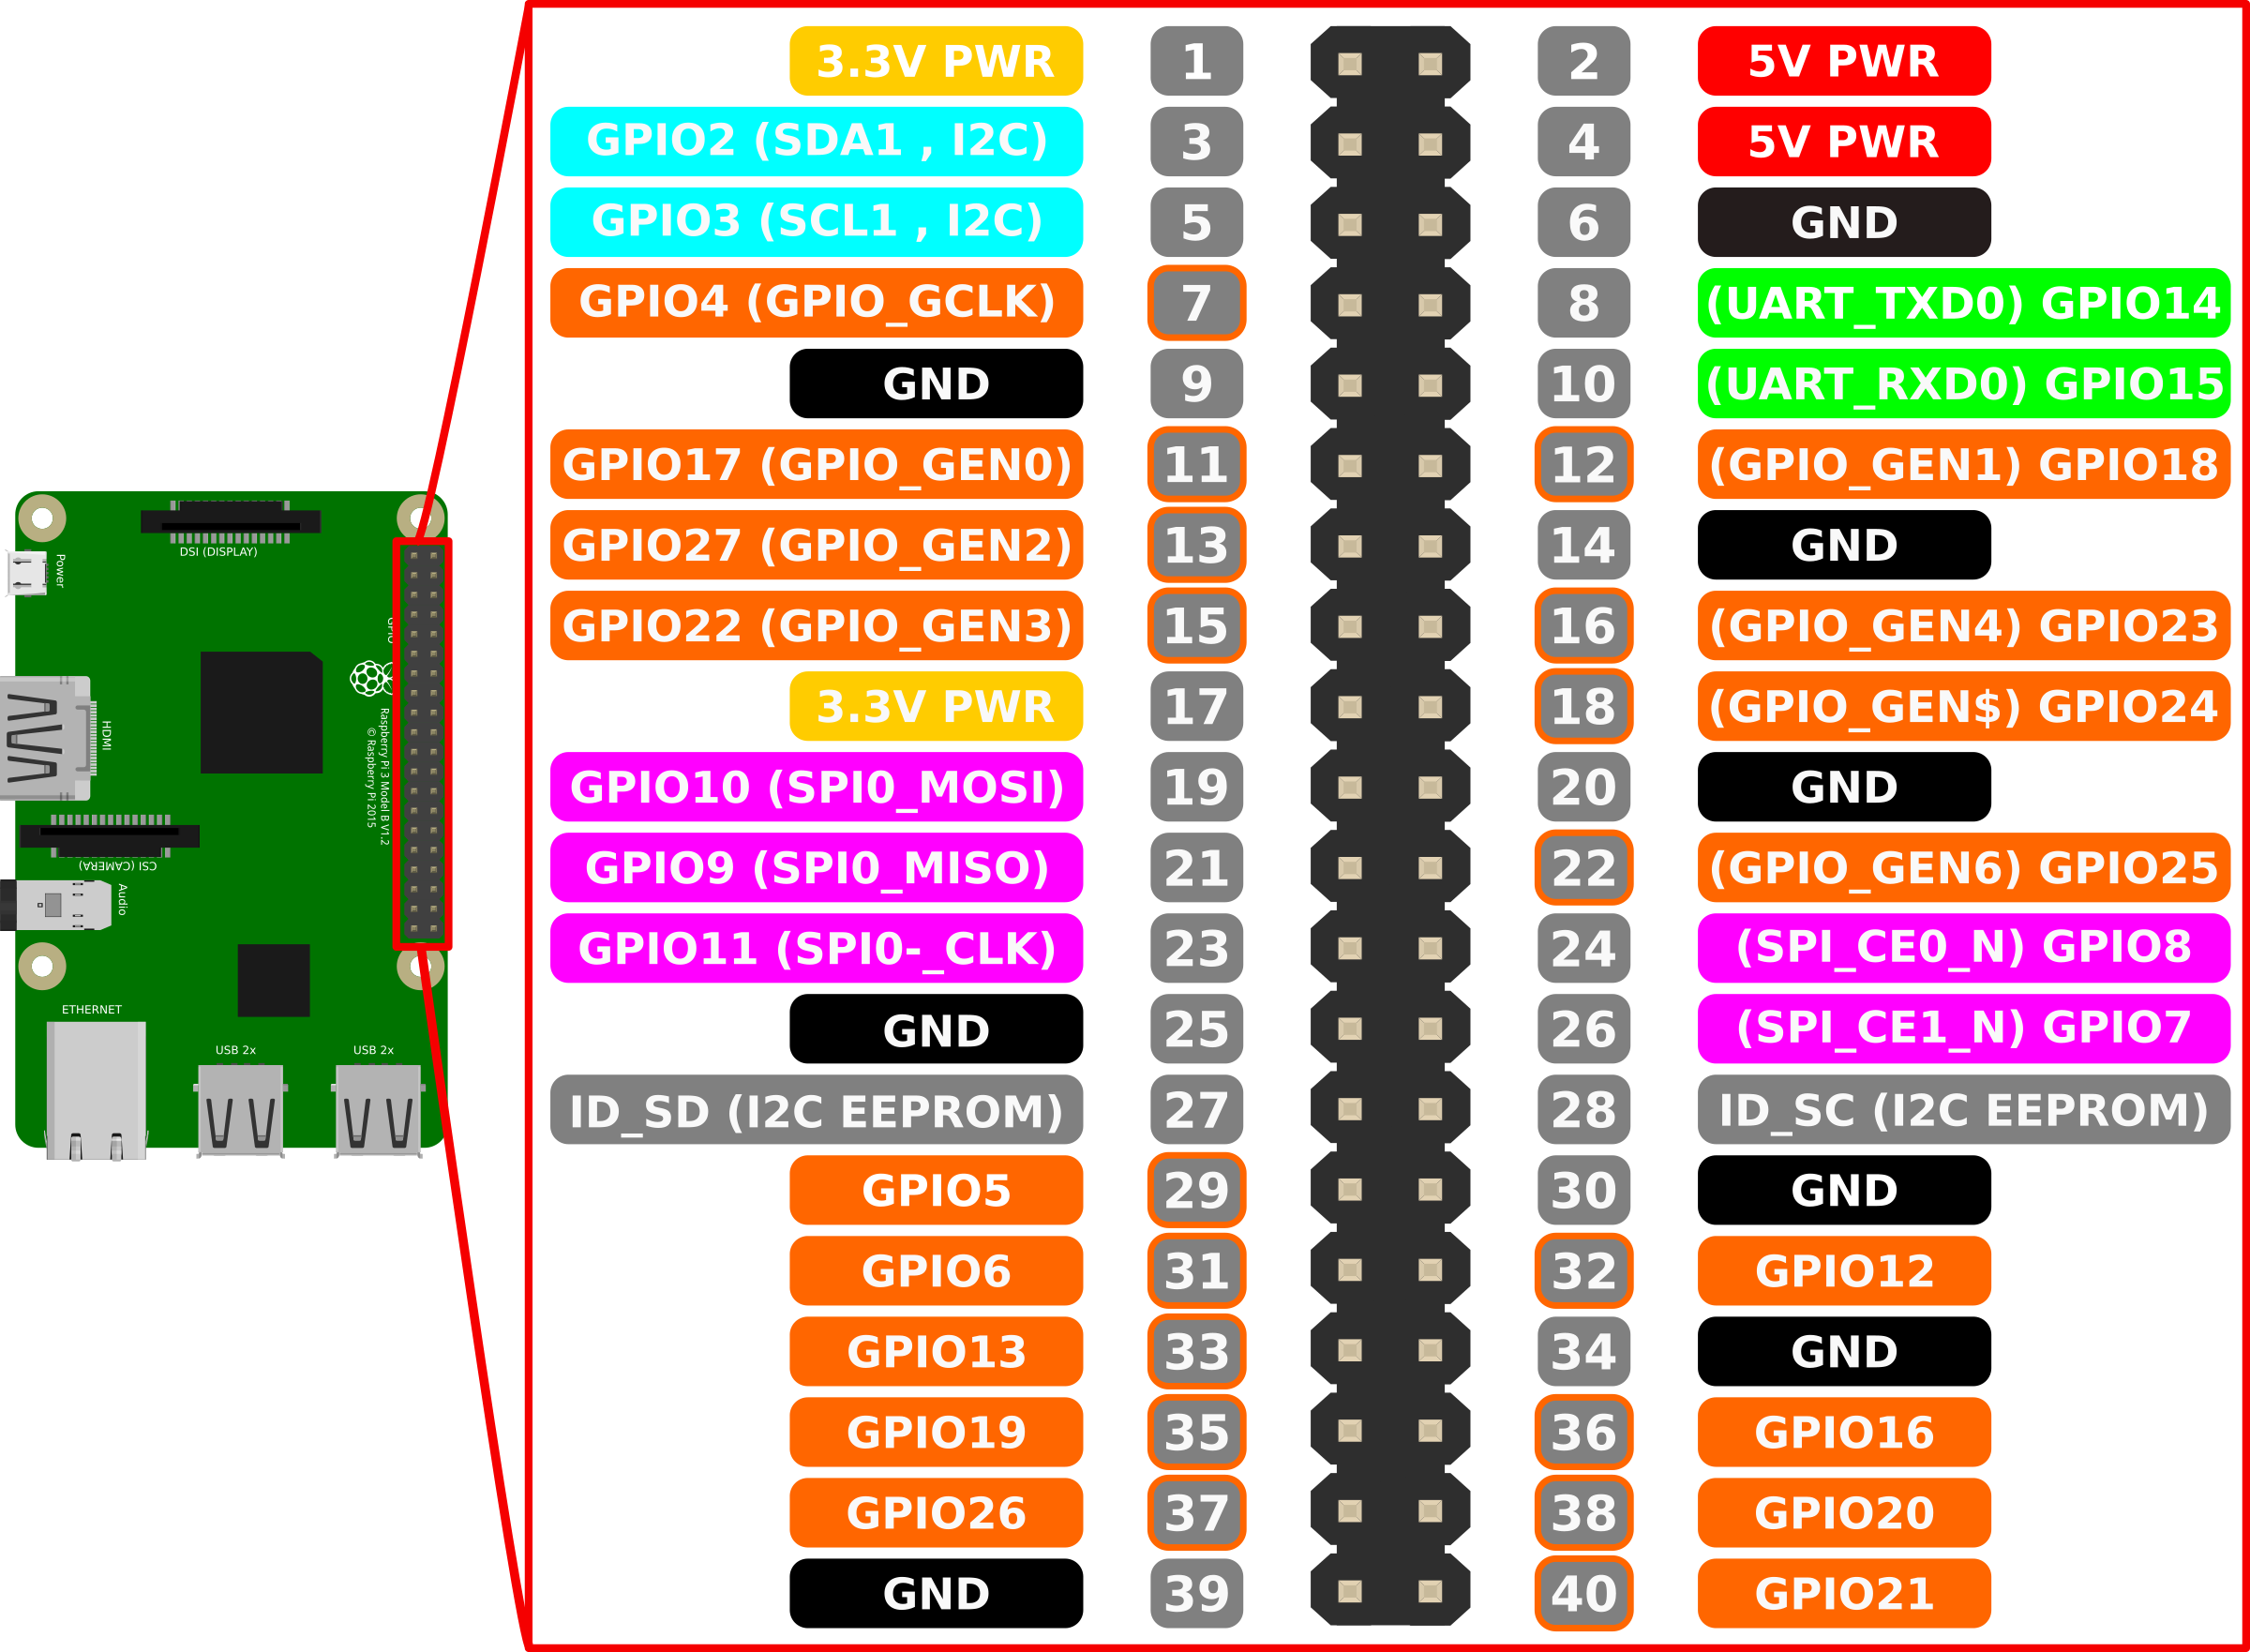
\includegraphics[width=0.8\textwidth]{img/frequem/rpi_gpio.png}\\
Raspberry Pi GPIO Layout \footcite{rpi_gpio}.
\end{center}

\subsection{Display}

Beim Display handelt es sich um ein 7 Zoll Exemplar von Waveshare, welches mittels HDMI an den Raspberry Pi angeschlossen wird. Wir entschieden uns für diese Größe, da sie unserer Meinung einen idealen Kompromiss zwischen Größe, um auf dem Gerät ordentlich arbeiten zu können und Portabilität, um es leicht transportieren zu können bietet. Das Display überzeugt mit einer für die Größe relativen hohen Auflösung von 1024x600 Pixel, diese Auflösung wäre zum Beispiel nicht möglich gewesen, wenn wir uns für einen Display entschieden hätten, welcher über die GPIO Pins des Raspberry angesteuert wird.\\
\\
Das HDMI Kabel musste modifiziert werden, um das ein- und ausschalten des Displays unabhängig von der Recheneinheit durchführen zu können. Es wurden jeweils die Litzen von Pin 12 und 18 entfernt, um die beiden Geräte elektrisch voneinander zu trennen. So kann mithilfe von Liestungs-NFETs bei jedem Gerät jeweils auf GROUND durchgeschalten werden um es mit Strom zu versorgen.\\

Ein HDMI-Kabel ist folgendermaßen aufgebaut (Pin 12 und 18 sind zu entfernen): 
\begin{center}
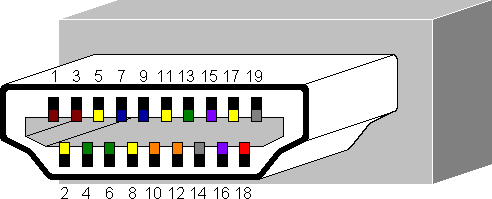
\includegraphics[width=0.7\textwidth]{img/frequem/hdmi_pins.png}\\
HDMI Male Typ A Pin Layout \footcite{hdmi_pinout}.
\end{center}

\subsection{Touchscreen}

Da es bei Touchscreens viele verschiedene Technologien gibt, welche heutzutage eingesetzt werden, war es nicht einfach einen passenden für unser Display-Modell zu finden.\\
\\
Unbedingt notwendig war, dass es sich um einen \textit{resistiven} Touchscreen handelt welcher mittels Druck funktioniert. Dadurch ist es möglich den Touchscreen mit einem Stift zu bedienen. Dies ist bei einem heutzutage üblichen \textit{kapazitiven} Touchscreen nicht möglich, da dieser nicht auf Druck sondern auf die Änderung der Kapazität reagiert.\\
\\
Wir entschieden uns für einen Touchscreen der Marke \textit{EETI}, der mittels USB an den Raspberry Pi angeschlossen werden kann, da für diesen offizieller Treibersupport zur Verfügung steht.\\
\\
Die Kalibrierung des Touchscreen wurde mithilfe des Tools xinput-calibrator durchgeführt.
\subsection{Power-Button}

Es war uns sehr wichtig, den Display und den Raspberry Pi durch einfaches Klicken eines Knopfes vom Strom trennen zu können, dies schränkt nicht nur den Stromverbrauch des Gerätes drastisch ein, es macht es auch möglich, den Display und Touchscreen unabhängig vom Raspberry Pi abzuschalten.\\

Wir setzten uns folgende Anforderungen für unseren Knopf:\\
\textit{Durch einfaches, kurzes Klicken auf den Knopf wird der Display ein- bzw. ausgeschaltet.
Durch längeres, dreisekündiges Halten des Knopfes und anschließendes Loslassen, wird die Recheneinheit ein- bzw. ausgeschaltet.}

Um diese Anforderungen umzusetzen nahmen wir einen \textit{Mikrocontroller} zur Hilfe. Wir entschieden uns für einen \textit{Arduino Pro Mini}, da dieser einen minimalen Energieverbrauch hat und leicht mit der Programmiersprache \textit{C} programmierbar ist.\\

Da es nicht möglich ist, sehr große Ströme mit dem Arduino allein zu schalten, verbauten wir für Display und Recheneinheit jeweils einen \textit{Leistungs-NFET}, der einen Strom von bis zu 3 Ampere schalten kann, ausreichend für unsere Zwecke also.\\\\

Weiters musste es möglich sein, dem Raspberry Pi ein Ausschaltsignal zu senden, welches ihn dazu bringt, sich selbst herunterzufahren um Korruption des Raspbian-Systems auf der Recheneinheit zu verhindern. Auch in die andere Richtung musste eine Signalleitung gelegt werden, die dem Mikrokontroller anzeigt, wenn der Raspberry Pi vollständig heruntergefahren ist, um ihn anschließend stromlos zu machen. Dazu wurde in jede Richtung jeweils ein \textit{NPN-Transistor} verbaut, um eine Brücke zwischen den 5 Volt des Arduino und den 3,3 Volt des Raspberry Pi herzustellen.\\

Um einen minimalen Leistungsaufwand des Mikrocontrollers zu garantieren wurde die LowPower-Library verwendet und mit Interrupts programmiert. Der Mikrocontroller schläft somit solange, bis der Knopf zum ein- und ausschalten betätigt wird.

\subsection{Akku}

Beim Akkumulator entschieden wir uns für 7 Stück 18650 Lithium-Ionen Zellen mit jeweils 2000 mAh. Wir trafen diese Entscheidung, da 18650-Zellen relativ häufig, zum Beispiel in Laptop-Akkus, vorkommen und eine hohe Energiedichte aufweisen.\\
\\
Mit einer Leistungsaufnahme von ca. 1,5 Ampere beim Raspberry Pi und ca. 1 Ampere beim Display kann man davon ausgehen dass der Akku für ca. 5,5 Betriebsstunden reichen wird. Bei einem Aufladestrom von 2,1 Ampere kann damit gerechnet werden, dass das Gerät, wenn vollkommen entladen, in einer Zeit von 6 Stunden vollständig aufgeladen werden kann. Diese Werte sind rein rechnerisch ermittelt worden, die eigentliche Betriebszeit ist dem Sachverhalt angemessen.\\
\\
Zum Laden und zur Energieabgabe an die einzelnen Komponenten haben wir uns für eine handelsübliche Powerbank der Marke RAVPower entschieden. Diese wurde für den Gebrauch von mehreren 18650-Zellen sowie zur andauernden Energieabgabe modifiziert. Eine solche Powerbank zu verwenden schien für uns der beste Weg zu sein, da die erreichte Effizienz beim Auf- und Entladen mit einfachen Elektronikbauteilen nicht erreichbar ist.\\
\\
Das Gerät ist mit einem Micro-USB Ladekabel aufzuladen, wir entschieden uns für diesen Anschluss da er heutzutage auf fast allen mobilen Geräten verbaut ist und somit die Wahrscheinlichkeit, bereits ein passendes Ladekabel zu besitzen relativ hoch ist.\\

\subsection{Gehäuse}

Beim Bau des Gehäuse gab es nicht viele Optionen, etwas zu verwenden, was bereits vorgefertigt war kam für uns nicht in Frage, nichts würde unseren Anforderungen entsprechen. Wir entschieden uns schließlich dafür unser Gehäuse selbst mittels CAD zu zeichnen und anschließend zu 3D-drucken.\\

\subsubsection{Modellierung}
Das modellieren der Ober und Unterteile wurde mithilfe der Free-Software FreeCAD durchgeführt. Da sich das Programm zur Zeit der Entwicklung noch in einem frühen Anfangsstadium befand, hatte ich mit einigen Abstürzen zu kämpfen. Nichts desto trotz gelang es mir Ober- und Unterseite des Gehäuses zu modellieren.\\
Folgende Modelle wurden erstellt:
\begin{center}
	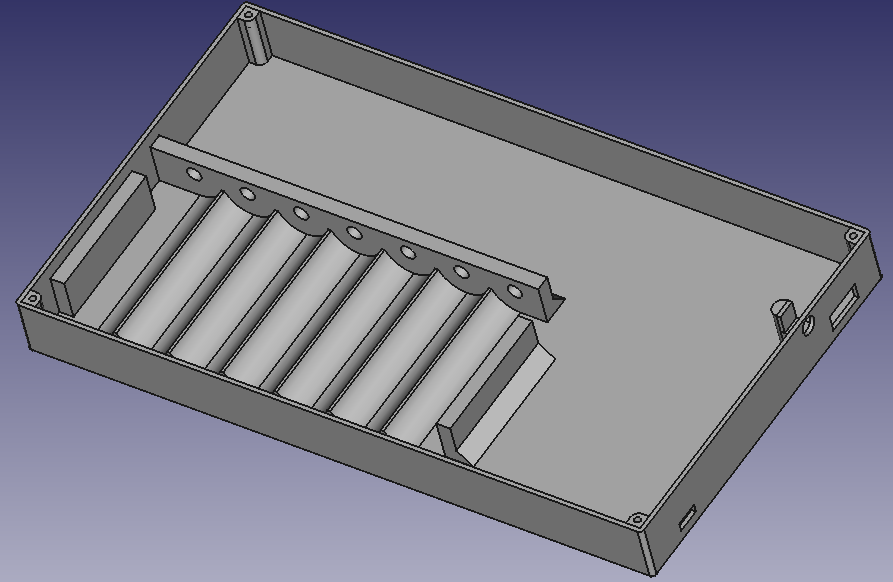
\includegraphics[width=0.7\textwidth]{img/frequem/model_bottom.png}\\
	Unterseite des Gehäuses\\
	
	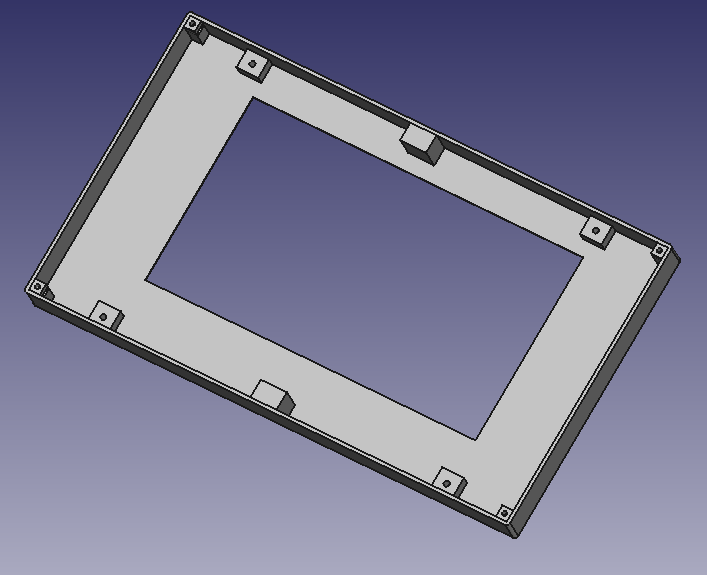
\includegraphics[width=0.7\textwidth]{img/frequem/model_top.png}\\
	Oberseite des Gehäuses\\
	
	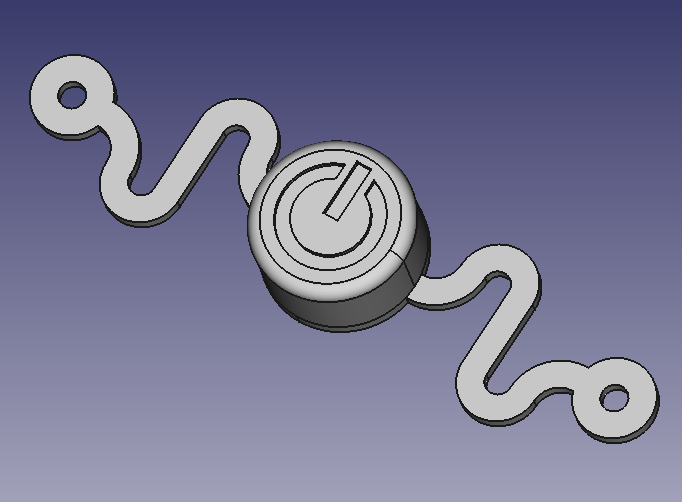
\includegraphics[width=0.7\textwidth]{img/frequem/model_button.png}\\
	Ein- und Ausschaltknopf\\
\end{center}

\subsubsection{3D-Druck}

Der 3D-Druck der einzelnen Gehäuseteile brachte einige Schwierigkeiten mit sich. Zuallererst waren Ober- und Unterseite des Gehäuse zu groß um auf dem uns zur Verfügung stehenden 3D-Drucker (Ultimaker 2+) gedruckt zu werden. Um dieses Problem zu beheben musste ich beide Seiten in jeweils zwei Hälften teilen und diese anschließend wieder zusammenfügen. Ich achtete bei diesem Prozess  darauf die 3D-Modelle so zu teilen, dass genügend Klebeflächen vorhanden waren um diese anschließend mit einen 2-Komponenten Epoxidkleber zusammenzukleben. Um eine stärkere Verbindung als nur auf den Klebeflächen zu erreichen klebte ich weiterhin Metallstreben an die Innenseiten des Gehäuses um dieses zusätzlich zu stabilisieren.\\
\\
3D-Drucken ist eine großartige Methode um schnell und effizient einen Prototypen eines Designs herzustellen. Der 3D-Drucker baut das gewünschte Werkstück auf, indem einzelne Kunststoff-Schichten nacheinander auf die sogenannte Build-Platform aufgetragen werden.\\
\\
Bei der Wahl des Kunststoffes gibt es zwei große Gruppen, welche oft verwendet werden: ABS und PLA. Wir entschieden uns unsere Modelle mit PLA zu drucken da dieser Kunststoff eine wesentlich einfachere Verarbeitung hat. Beim Drucken von ABS kommt es oft zu unkontrollierten Verformungen und das Werkstück ist oft verzogen. Ein Vorteil von ABS allerdings ist, dass sich der Kunststoff mithilfe von Aceton leicht anätzen lässt, was zu einer schöneren Oberfläche führt. Da wir aber unser Gehäuse sowieso vorhatten zu lackieren entschieden wir uns schließlich für PLA.\\
\\
Um ein Modell 3D-drucken zu können muss es vorher in GCODE umgewandelt werden. Dieser GCODE besteht aus einzelnen Instruktionen welche vom Drucker der Reihe nach ausgeführt werden. Dieser Prozess, das sogenannte Slicing wurde mithilfe der Software Cura durchgeführt. Wir entschieden uns für einen Füllgrad von 10 \% da dies für die Zwecke eines Gehäuses durchaus reicht und wir dadurch Kunststoff sparen konnten.\\
\\